\documentclass{article}
\usepackage[utf8]{inputenc}
\title{lab 3: lasso, ridge and elastic nets a deeper dive }
\author{wbg231 }
\date{December 2022}
\newcommand{\R}{$\mathbb{R}$}
\newcommand{\B}{$\beta$}
\newcommand{\A}{$\alpha$}
\newcommand{\D}{\Delta}

\newcommand{\avector}[2]{(#1_2,\ldots,#1_{#2})}
\newcommand{\makedef}[2]{$\textbf{#1}$:#2 }
\usepackage{tikz,graphicx,hyperref,amsmath,amsfonts,amscd,amssymb,bm,cite,epsfig,epsf,url}

\begin{document}

\maketitle

\section{introduction}
\begin{itemize}
\item why is feature normalization important during regularization? it allows us to keep the magnitude of our features a. standard across different variables. and b. small so they are less effected by changes in the input data 
\section{repeated features}
\subsection{a very simple model}
\item suppose we have one feature $x_1\in \mathbb{R}$
\item and some response variable $y\in \mathbb{R}$
\item suppose we got some data and ran least squares linear regression and the ERM came out as $$\hat{f}(x_1)=rx_1$$
\item what happens if we add a new feature $x_2$ that we know $x_2=x_1$
\subsection{duplicate features}
\item the new feature $x_2$ gives us no new information 
\item so the erm is still $$\hat{f}(x_1,x_2)=4x_1$$, but as we know $x_1=x_2$
\item we can also write the following as valid erm $\hat{f}(x_1,x_2)=2x_1+2x_2$, $\hat{f}(x_1,x_2)=x_1+3x_2$, $\hat{f}(x_1,x_2)=4x_2$
\item we can try to decide between these by introducing $\ell_{1}$ or $\ell_{2}$ regularization 
\subsection{duplicate features with norms}
\item $\hat{f}(x_1,x_2)=w_1x_1+w_2x_2$ is an ERM $\iff w_1+w_2=4$
\item so consider the $\ell_{1}$ and $\ell_{2}$ norms for various solutions 
\item 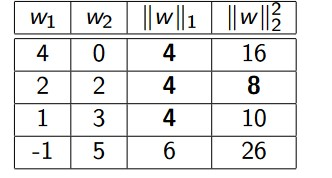
\includegraphics[width=10cm]{labs/lab_3/images/r3_1.jpg}
\item $\ell_{1}$ does not care which solution is chosen as long as they have the same sign 
\item $\ell_{2}$ just wants the weights to be spread out evenly 
\subsection{equal features in L_2 constraint }
\item 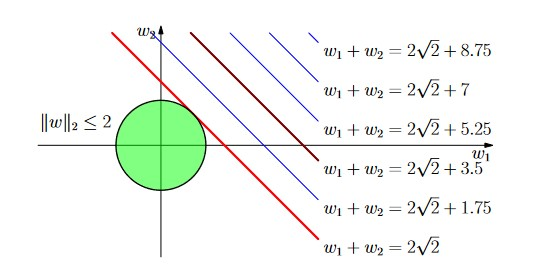
\includegraphics[width=10cm]{labs/lab_3/images/r3_2.jpg}
\item suppose that the brown line corresponding to the ERM
\item empirical risk increases as we move away from these parameter settings 
\item so intersection of our objective function and the norm ball is the ridge solution, note however that this occurs at $w_1=w_2$
\subsection{equal features with the l  1 constraint}
\item 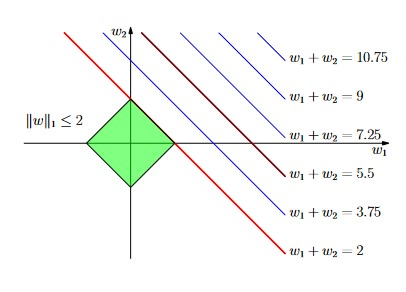
\includegraphics[width=10cm]{labs/lab_3/images/r3_3.jpg}
\item note that the lasso solution in this case is the set $\{ (w_1,w_2): w_1+w_2=2, w_1,w_2\geq 0)\}$ ie just values that are both positive and sum to 2. 
\section{linearly dependent features}
\subsection{linearly related features}
\item given we have a linear prediction function $f(x)=w_1x_1+w_2x_2$
\item suppose that $x_2=2x_1$
\item then all the functions with $w_1+2w_1=k$ are the same in the unconstrained erm perspective
\item what function will we selects if we ERM with $\ell_{1},\ell_{2}$
\item compare a solution that just uses $w_1$ to a solution that just uses $w_2$
\subsection{linearly related features l2}
\item so note our level curves are now $w1+2w_2=c$ so this will intersect with our $l_2$ constraint at $w_2=2w_1$
\subsection{linearly related features with an l1 constraint}
\item 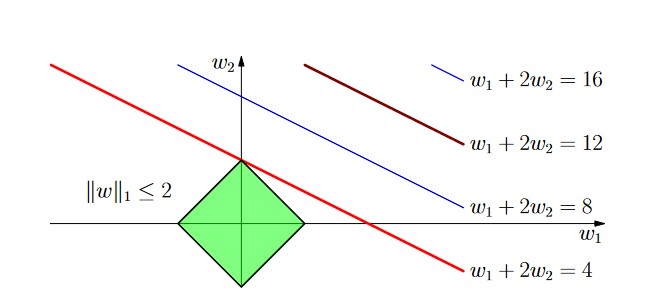
\includegraphics[width=10cm]{labs/lab_3/images/r3_4.jpg}
\item so note that our features $x_2=2x_1$ so in other words $w_1$ in effect vies us the same information with a smaller weight 
\item thus we are going to take a spare solution with just $w_2$

\subsection{take away}
\item for identical features
\begin{itemize}
    \item $\ell_{1}$ regularization spreads the weights arbitrarily as long as they have the same sign 
    \item $\ell_{2}$ regularize chooses the weights evenly
\end{itemize}
\item for linearly dependant features
\begin{itemize}
    \item $\ell_{1}$ will chose the viable with larger scale, and st the wight of others to zero
    \item $\ell_{2}$ prefers the variable with larger scales, and spreads the wight proportionally to the scale. 
\end{itemize}
\subsection{empirical risk for square loss and linear predictors}
\item for square loss and linear predictors, sets of w giving the same empirical risk from ellipsoids around the ERM
\item with $x_1, x_2$ linearly related $X^{t}X$ has a zero eigen value and thus no inverse 
\item so our optimal set is no longer an ellipsoid it is instead a degenerate ellipsoid that looks like a line, 
\end{itemize}
\section{correlated features}
\subsection{correlated features with the same scale}
\item suppose $x_1, x_2$ are highly correlated with the same scale
\item this is quite typical in data after normalization 
\item there is nothing degenerate here so the level sets are ellipsoids
\item but the higher the correlation the closer we get to generate we get 
\item that is ellipsoids keep stretching out towards parallel lines
\subsection{co-related features l1 reg}
\item 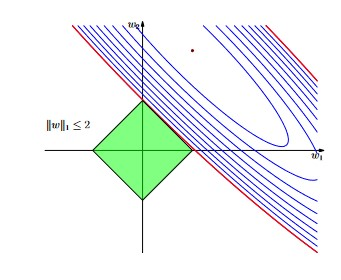
\includegraphics[width=10cm]{labs/lab_3/images/r3_5.jpg}
\item with line like ellipses that come with highly correlated features, $\ell_{1}$ will just pick anything on the top right edge
\item this means minor changes in our data Can lead to a very different intersection wights 
\item further this makes devotion between weighs with the same scale seem kind of arbitrary
\subsection{a case against sparsity}
\item suppose there is some unkown value $\theta \in \mathbb{R}$
\item we get 3 noise observations of $\theta$ $x_1,x_2,x_3 \sim N(0,1)$ sand are idd 
\item what is a good estimator$\hat{\theta}$ of $\theta$
\item would you prefer $\hat{\theta}=x_1$ or $\hat{\theta}=\frac{1}{3}(x_1+x_2+x_3)$? the second one since it averages the randomness
\subsection{estimator preform acne analysis}
\item $E[x_1]=\theta$, $E[\frac{1}{3}(x_1+x_2+x_3)]=\theta$ so both are unbiased
\item $var(x_1)=1$
\item $var(\frac{1}{3}(x_1+x_2+x_3)=\frac{1}{9}var(x_1,x_2,x_3)=\frac{1}{9}3=\frac{1}{3}$
\item so average has a smaller variance since error cancels its self out more 
\item this holds for more features, so in other words when we have highly correlated features we can reduce variance by keeping more of them as opposed to predicting with just 1. 
\subsection{example with highly correlated features}
\item model in words
\begin{itemize}
    \item y is some unknown lienar combination of $z_1,z_2$
    \teim but we do not observe $z_1,z_2$ directly
    \item we get three noisy observations of $z_1$ called $x_1,x_2,x_#$ and three noisy observations of $z_2$ called $x_4,x_5,x_6$
    \item we want to predict y form our noise observation 
    \item that is we want an estimator $\hat{y}=f(x_1,x_2,x_3,x_4,x_5,x_6)$ for estimating y 
    \item suppose $(x,y)$ generated as follows $z_1,z_2 \sim n(0,1)$ independent and $\epsilon_0,\epsilon_1,\epsilon_2, ...x\epsilon_6 \sim n(0,1)$
    \item thus $y=3z_1-1.5z_2+2\epsilon_{0}$
    \item and $x_j=z_1+\frac{e_{j}}{5}$ for j in [1,3] and $x_j=z_2+\frac{\epsilon_{j}}{5}$ for j in 4,5,6
    \item suppose we generated 100 samples of $(x_1..x_6), y$ pairs
    \item the co relation with in the group of x's is around .97
    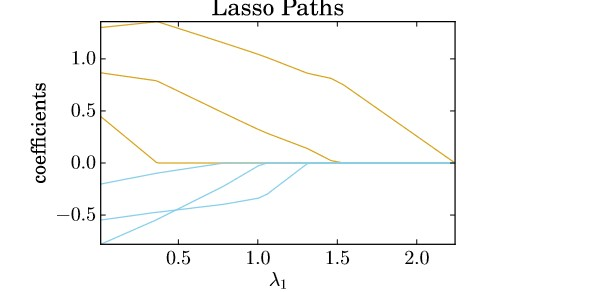
\includegraphics[width=10cm]{labs/lab_3/images/r3_6.jpg}
    \item where lines of the same color correspond to features with correlated info
    \item distribution of weighs among the features seems kind of arbitrary. 
\subsection{hedge bet when variables are highly co related }
\item when variables are highly co related ( and have the same scale assuming we have standardized features) we want to give them roughly the same weight 
\item why? because it lets the errors can cl out 
\item how can we have the weight spread out more evenly?
\section{elastic nets}
\item the elastic net combines the lasso and ridge penalty $$\hat{w}=armin_{w\in \mathbb{R}^{d}}(w^tx_u-y_i)^2+\lambda_1||w||_1+\lambda_2||w||_2^2$$
\item we expect correlated random features to have similar coefficients 
\subsection{highly correlated features, elastic nets }
\item 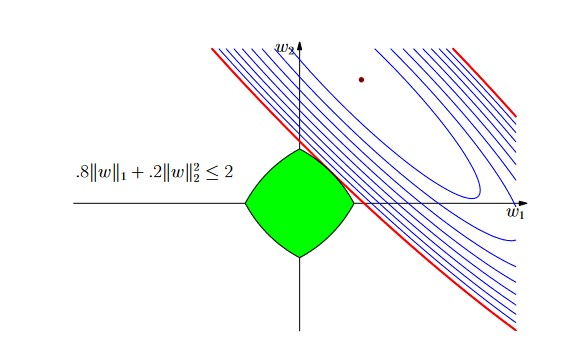
\includegraphics[width=10cm]{labs/lab_3/images/r3_7.jpg}
    \item given $\lambda_1=.8,\lambda_2=.2$ we will have this kind of shape that is a slightly rounded diamond, this leads to an elastic net solution closer to $w_2=w_1$ line despite high correlation of features
\subsection{elastic net path}
\item 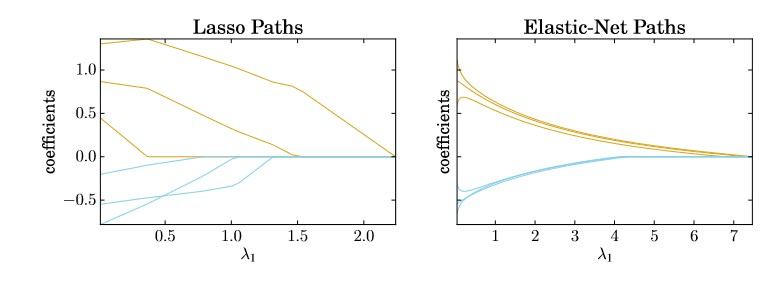
\includegraphics[width=10cm]{labs/lab_3/images/r3_8.jpg}
\item the ratio of weights is much less arbitrary
\item 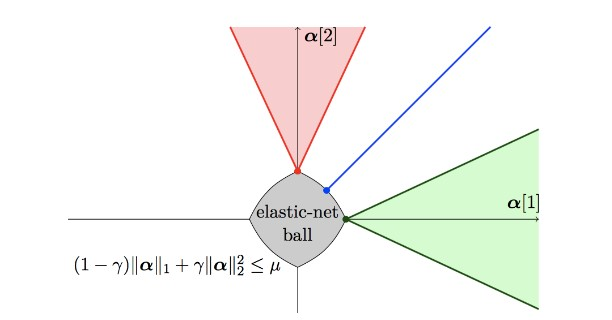
\includegraphics[width=10cm]{labs/lab_3/images/r3_9.jpg}
\item the green and red area are closest to the spare solution, but everywhere else would lead to a non-coroner case. so both have a pretty sizeable likelihood of happening 

\end{itemize}
\end{document}
